\ylDisplay{Kaks kuulikest} % Ülesande nimi
{EFO žürii} % Autor
{piirkonnavoor} % Voor
{2018} % Aasta
{P 3} % Ülesande nr.
{2} % Raskustase
{
% Teema: Mehaanika

\ifStatement
Kaks kuulikest alustavad samaaegselt võrdsete kiirustega liikumist mööda joonisel näidatud pindu. Kumma kuulikese kiirus on punkti $B$ jõudes suurem või on nende kiirused võrdsed? Kumb kuulike jõuab punkti $B$ varem või jõuavad nad punkti $B$ samaaegselt? Hõõrdejõudu pole vaja arvestada. Põhjendage vastust.
\begin{center}
	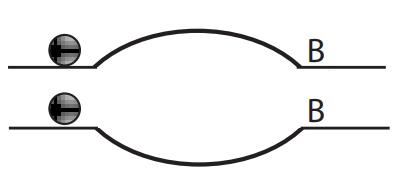
\includegraphics[width=0.5\linewidth]{2018-v2p-03-yl.PNG}
\end{center}
\fi

\ifHint
Kui joonestada graafik kiiruse ja aja vahelisest seosest, siis teepikkus graafikul on võrdne graafiku joone aluse viirutatud pindalaga.
\fi

\ifSolution
\begin{center}
	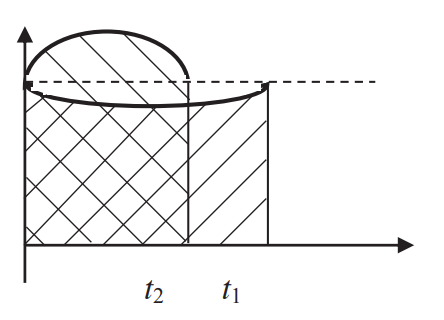
\includegraphics[width=0.5\linewidth]{2018-v2p-03-lah.PNG}
\end{center}
Kuulikeste kiirused on punkti $B$ jõudmisel võrdsed, sest künka ja lohu kumerused on sarnased ning teepikkused on võrdsed. Esimese kuulikese kiirus esialgu väheneb ja siis suureneb, teisel vastupidi. Ajavahemiku, mis kulub kuulikestel punkti $B$ jõudmiseks saab kiiruse graafikult. Teepikkus graafikul on võrdne graafiku joone aluse viirutatud pindalaga. Pindalade võrdsusest selgub, et $t_2 < t_1$.
\fi
}
